\documentclass[12pt]{article}

\usepackage[vmargin=1in,hmargin=1in]{geometry}
\usepackage{amsmath}
\usepackage[parfill]{parskip}
\usepackage{hyperref}
\usepackage{natbib}
\usepackage{bm}
\usepackage{amsfonts}
\usepackage{graphicx}
\usepackage{abstract}
\usepackage{lineno}
\usepackage{setspace}

\hypersetup{pdfstartview={Fit},hidelinks}


\usepackage{caption}
\captionsetup[figure]{labelformat=empty}% redefines the caption setup of the figures environment in the beamer class.


\title{Ecology Appendix S2 \\ Simulation study accompanying the paper: \\ \it Modeling abundance, distribution, movement, and space
  use with camera and telemetry data}
\author{Richard B. Chandler$^1$\footnote{Corresponding author: rchandler@warnell.uga.edu}, Daniel A. Crawford$^2$, Elina P. Garrison$^3$, \\
  Karl V. Miller$^1$, Michael J. Cherry$^2$}

\begin{document}



\maketitle

\vspace{12pt}

\begin{description}%[labelindent=1pt]%[leftmargin=1cm]%,labelwidth=\widthof{\bfseries Example:}]
%  \large
\item[$^1$] Warnell School of Forestry and Natural Resources, University of Georgia %\\
\item[$^2$] Caesar Kleberg Wildlife Research Institute at Texas A\&M University-Kingsville %\\
\item[$^3$] Florida Fish and Wildlife Conservation Commission %\\
\end{description}

\clearpage

\section*{Introduction and Methods}

We conducted a small simulation study to evaluate the performance of the
spatial capture-recapture model with an explicit movement process
described in the manuscript.
The design and parameter values were chosen to resemble the estimates
from the deer example in the manuscript. A uniform capture process was
simulated to resemble aerial capture and transmitter
deployment. The camera design in the simulation study was the same as
in the deer example, with 60 cameras spaced by 200--500 m. We simulated
90 occasions and used a fix rate of 1 location every 3
occasions. Parameters (defined in the manuscript) were $N=100$,
$p^{\mathrm cap}=0.25$, $\lambda_0=2$, $\sigma^{\mathrm det}=50$,
$\sigma^{\mathrm move}=600$. We 
considered 5 scenarios in which the autocorrelation parameter ($\rho$)
of the Ornstein-Uhlenbeck movement model was assigned values: 0.55,
0.65, 0.75, 0.85, and 0.95. 

For each scenario, we simulated 100 datasets and fit both
the data generating model (SCR-move) and a mis-specified SCR model
(SCR0) with no movement process. Inference was made using 10,000 MCMC
samples from the joint posterior following a 2,000 iteration
burn-in. Code to reproduce the simulation study can be found at
\url{https://github.com/rbchan/scr-move/R/sims}.

% \begin{table}[h!]
%   \centering
  
%   \caption{Scenarios considered in the simulation study}
%   \label{tab:sims}
% \end{table}


\section*{Results and Discussion}

The number of individuals captured and outfitted with telemetry
devices ranged from 13--35 in the simulated datasets. As with the deer
example, only a small fraction (ranging from 0--10) were detected by
cameras. 

Bias was reduced in all 5 cases when switching from the SCR0 model to
the SCR-move model (Fig.~\ref{fig:bias}). Improvement in bias ranged
from 2--6\%. Bias of the SCR+move model was $\le2\%$ for the first two
scenarios. For the other three scenarios (with 
$\rho=$0.75, 0.85, and 0.95), bias of the SCR+move model was
5--8\%, although some of this was likely attributable to Monte Carlo
error resulting from the small number of simulated datasets.
Coverage of 95\% credible intervals was close to 0.95 for
the SCR+move model in all scenarios and was better than the SCR0 model
(Fig.~\ref{fig:bias}). Variance of the estimator was greater for the
SCR+move model than for the mis-specified SCR0 model.


\clearpage

\begin{figure}[h!]
  \centering
  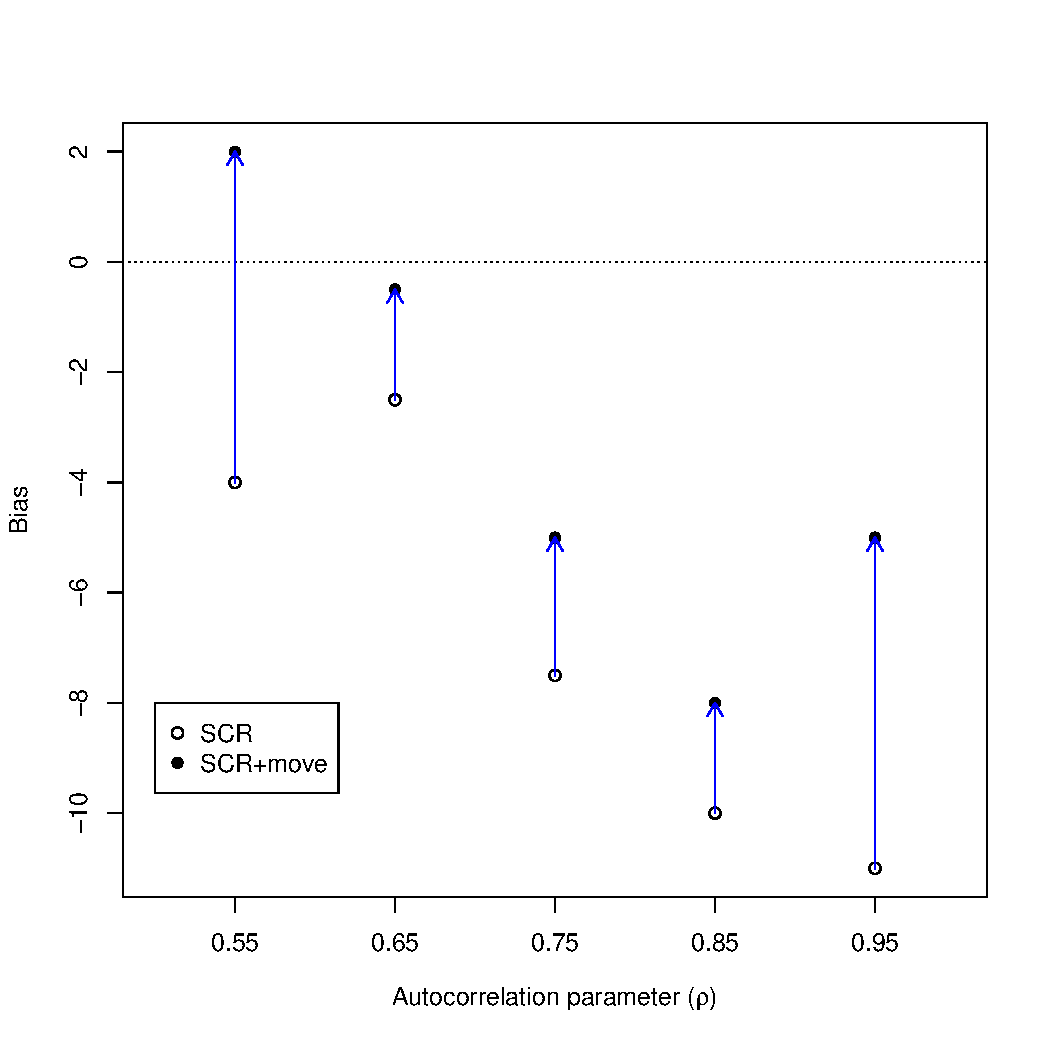
\includegraphics[width=0.5\textwidth, trim=0mm 15mm 0mm 15mm, clip]{../R/sims/bias-N.pdf} \\
  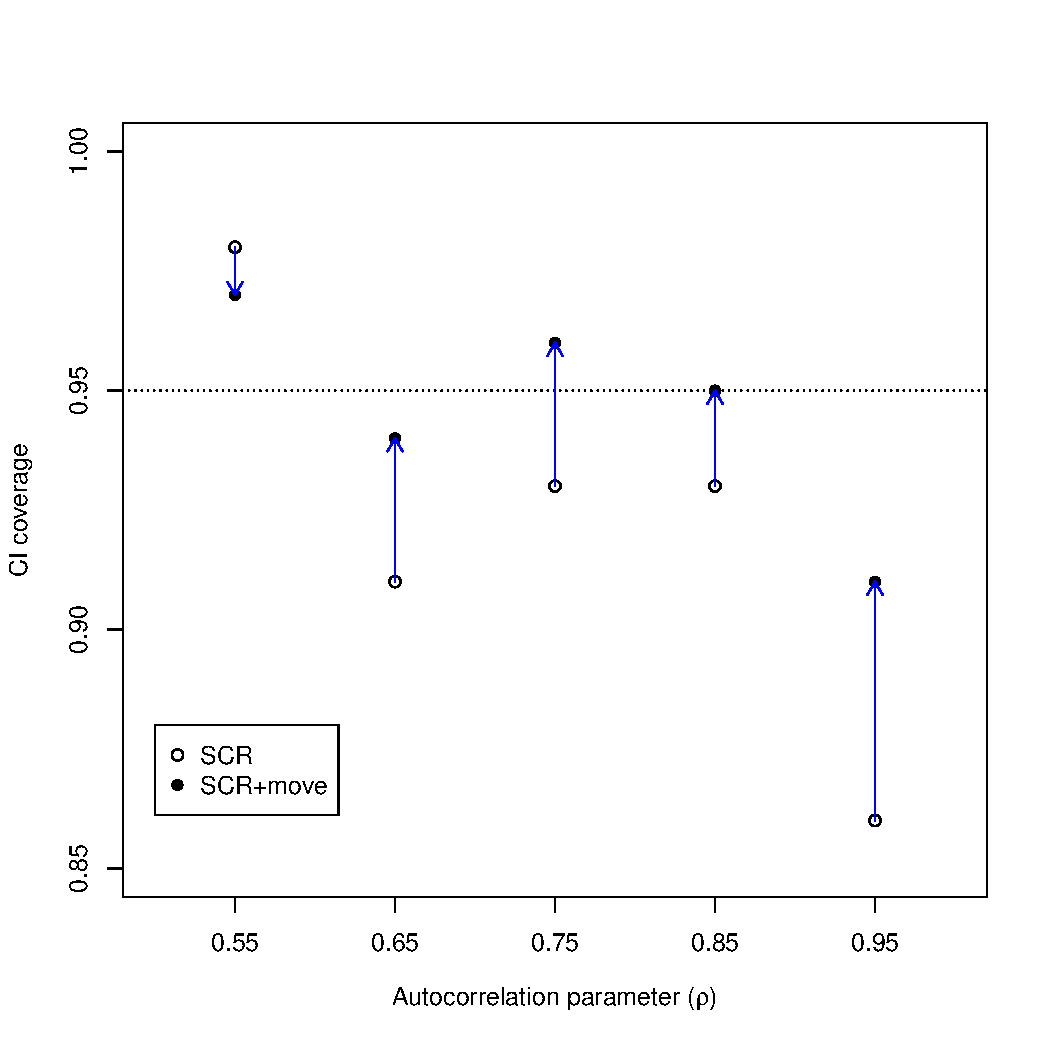
\includegraphics[width=0.5\textwidth, trim=0mm 15mm 0mm 15mm, clip]{../R/sims/cover-N.pdf} \\
  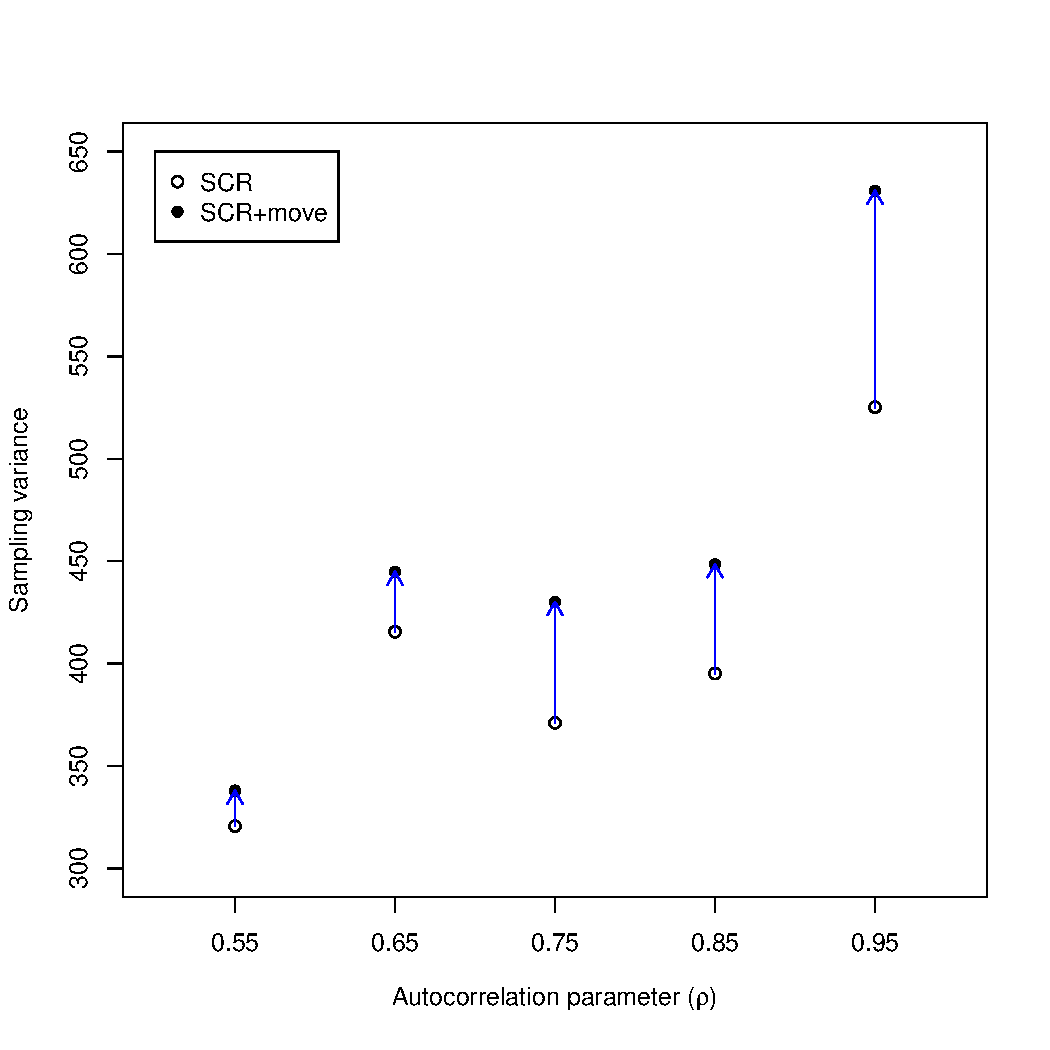
\includegraphics[width=0.5\textwidth, trim=0mm 0mm 0mm 15mm, clip]{../R/sims/var-N.pdf}
  \caption{Figure S1. Bias, 95\% CI coverage, and variance of the posterior mode
    as a point estimator of population size ($N$) under five values of
    the parameter $\rho$ controlling autocorrelation in movement. The
    data generating value of abundance was $N=100$. } 
  \label{fig:bias}
\end{figure}



\end{document}


